\documentclass[11pt]{article}

\usepackage[utf8]{inputenc}
\usepackage[T1]{fontenc}
\usepackage[margin=1.1in]{geometry}
\usepackage{amsmath,amssymb}
\usepackage{booktabs}
\usepackage{graphicx}
\usepackage{natbib}
\usepackage{hyperref}
\hypersetup{colorlinks=true,linkcolor=blue,citecolor=blue,urlcolor=blue}
\usepackage{caption}
\captionsetup{font=small,labelfont=bf}

\title{\textbf{The Hidden Options Market}\\[0.4em]
\large FLEX Inventory in Clearing Data, and Whether It Predicts the Visible Market}

\author{Anonymous\thanks{Independent research. REDACTED did not fund,
sponsor, approve, or endorse this work. The affiliation records the author's status as
a student only, and the views expressed are the author's alone.
Correspondence: \texttt{REDACTED}.}\\[0.3em]
\textbf{REDACTED}}

\date{19 August 2026}

\begin{document}
\maketitle

\begin{abstract}
\noindent
FLEX options are negotiated bilaterally, cleared centrally, and absent from the listed
option chains on which most empirical option research is built. The Options Clearing
Corporation publishes a daily FLEX open-interest report, and we use it to assemble a
panel of 269 activity dates, 1,691 underlyings and 9.1 million series-days. The market
is large and growing fast: open interest roughly doubled over the panel, from 34.8 to
73.0 million contracts, and mark value rose from \$319bn to \$596bn. It is also
concentrated and short-dated --- the ten largest underlyings hold 29\% of open
interest, and 56\% of it expires within sixty days. We then ask whether this hidden
inventory predicts the visible market, and find that it does not: per-underlying
inventory innovations carry no information about next-day or next-fortnight realised
volatility, with a placebo using inventory dated \emph{after} the outcome returning the
same coefficient and the same $t$-statistic to two decimal places. Along the way we
report two measurement results with wider application. First, a natural
identification heuristic --- treating strikes off the standard listing grid as FLEX ---
achieves precision $0.67$ and recall $0.34$ against the authoritative report, missing
two thirds of FLEX because FLEX is frequently struck on the grid. Second, treating
cleared series as economic positions mismeasures them severely and in both directions:
a butterfly counted leg by leg is credited with 49 times its maximum attainable value,
a four-leg collar is counted three times over, and a synthetic long call struck at
\$1.87 against a \$765 spot is recorded at \$7m when its exposure is \$2.9bn.

\vspace{0.8em}
\noindent\textbf{Keywords:} FLEX options; clearing data; open interest; hidden
inventory; dealer hedging; option market structure.

\noindent\textbf{JEL:} G13, G14, G23.
\end{abstract}

\section{Introduction}

Most empirical work on option markets observes the listed chain: the set of
exchange-listed series with continuously disseminated quotes. FLEX options are not in
it. They are negotiated bilaterally, with strike, expiry and exercise style chosen by
the counterparties, and then submitted for central clearing. They do not print on the
consolidated tape and they do not appear in chain data.

They are nonetheless publicly reported. The Options Clearing Corporation publishes a
daily FLEX open-interest report --- one for equity classes and one for index classes
--- giving symbol, right, expiry, strike, mark price and open interest for every
cleared FLEX series, with roughly twenty months of history. We are not aware of
systematic empirical work using it.

This paper assembles that report into a panel and asks what is in it and whether it
matters.

\paragraph{What the market looks like.} It is large, fast-growing, concentrated and
short-dated. Across 269 activity dates ending 17 August 2026, open interest roughly
doubled, from 34.8 to 73.0 million contracts, and the mark value of that inventory rose
from \$319bn to \$596bn. On the final date, 42,740 series across 1,023 underlyings carry
73.0 million contracts; the largest ten underlyings account for 29\% of it, 56\% of
open interest expires within sixty days, and calls are 57\% of the total.

\paragraph{Whether it predicts anything.} The economic reason to care is that a dealer
taking the other side of a FLEX trade hedges it in the listed market and carries the
residual convexity for the life of the position. If that is material, inventory
observed at date $T$ --- published overnight, and so available at $T+1$ --- should carry
information about what follows.

It does not, at least at the resolution available here. Per-underlying inventory
innovations do not predict next-day absolute or squared returns, nor mean absolute
returns over the following three, five or ten days. The estimate that comes closest is
$t=-1.37$ on next-day absolute return. A placebo using inventory dated \emph{after} the
outcome, which cannot carry information by construction, returns the same coefficient
and the same $t$-statistic to two decimal places. Whatever links inventory to
volatility runs equally well backwards in time.

We report the null rather than the marginal coefficient because the placebo is what
distinguishes them, and on a smaller panel the same predictor reached $t=-1.95$ --- a
value that, without the placebo, would have been reportable as suggestive.

\paragraph{Two measurement results.} Both emerged from building the census and both
apply beyond FLEX.

The first concerns identification. Before locating the authoritative report we
identified FLEX indirectly, reasoning that listed strikes fall on a standard grid so an
off-grid strike must be FLEX. Scored against the report, that heuristic achieves
precision $0.67$ and recall $0.34$: it misses two thirds of FLEX, because FLEX is
frequently struck \emph{on} the grid, and a third of what it flags is not FLEX. We
report this because the reasoning is natural and the failure is not visible without
ground truth.

The second concerns counting. Open interest is reported per series; a position is not a
series. Conflating them produced errors of 49-fold, threefold, and three orders of
magnitude, with opposite signs that do not cancel. Any study using open interest is
exposed to the same conflation.

\paragraph{Relation to the literature.} Work inferring option-market positioning from
listed data must assume who holds each side: \citet{bollen2004} read net buying pressure
from the implied volatility function, \citet{garleanu2009} model demand pressure and
estimate it from data identifying end users and intermediaries, and \citet{ni2005} use
strike-level open interest to identify price clustering at expiration. Each takes the
observable series set as given. We add a category of series that listed data omits, and
show that a natural way to find it without the authoritative source fails. We do not
solve the sign problem, and our inventory measures are gross throughout.
\citet{park2025} study option-income funds, one of the identifiable users of FLEX; our
panel places them within the wider market.

\section{Data}

\subsection{The report}

OCC's FLEX open-interest report is fixed-layout text carrying, for each cleared FLEX
series: root, right, expiry, strike, mark price and open interest, grouped by option
class with per-class totals. FLEX roots are the listed root with a numeric prefix
(\texttt{1AAL}, \texttt{2DJX}, \texttt{4SPY}), which identifies them exactly.

We parse both the equity and index reports and validate each against the totals the
report itself carries. On the reference date all 1,184 class totals reconcile.

Files are stored under the report's own activity date rather than the date they were
fetched. This is not pedantry: OCC publishes overnight, so a capture taken during a
session returns the previous settlement, and two of our early captures were
byte-identical across 113,610 series for exactly this reason. Partitioning by capture
date would have entered one settlement into the panel twice as two apparently stable
days.

\subsection{The panel}

The panel covers 269 activity dates from 23 July 2025 to 17 August 2026, 1,691
underlyings and 9,056,242 series-days.

\begin{table}[t]
\centering
\caption{The FLEX market over the panel, and its composition on the final date.}
\label{tab:panel}
\begin{tabular}{lrr}
\toprule
& Start (2025-07-23) & End (2026-08-17) \\
\midrule
Open interest (m contracts) & 34.8 & 73.0 \\
Mark value (\$bn) & 319 & 596 \\
\midrule
\multicolumn{3}{l}{\emph{Final date}} \\
Series & & 42,740 \\
Underlyings & & 1,023 \\
Top 10 underlyings, share of open interest & & 29.2\% \\
Open interest expiring within 60 days & & 55.9\% \\
Calls, share of open interest & & 57.2\% \\
\bottomrule
\end{tabular}
\end{table}

Open interest roughly doubled over thirteen months and mark value rose by 87\%
(Figure~\ref{fig:growth}). The five largest underlyings on the final date are SPY, SPX,
one large-cap technology name, an index product and one further single name.

\begin{figure}[t]
\centering
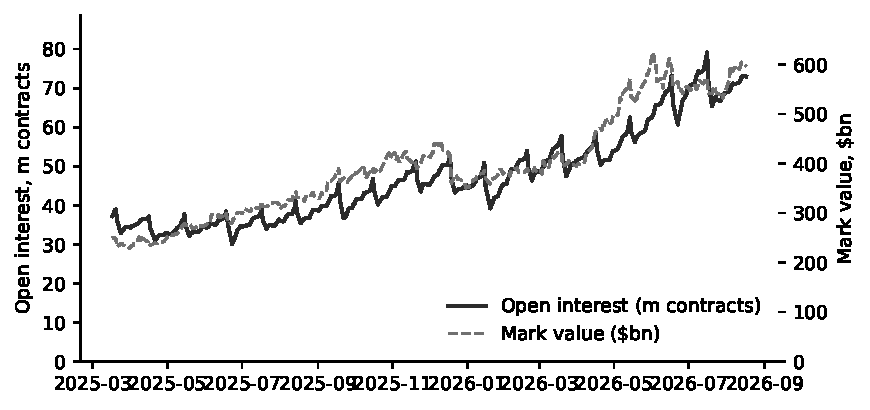
\includegraphics[width=0.86\textwidth]{figures/growth.pdf}
\caption{FLEX open interest and its mark value across the panel. Both roughly double.}
\label{fig:growth}
\end{figure}

\begin{figure}[t]
\centering
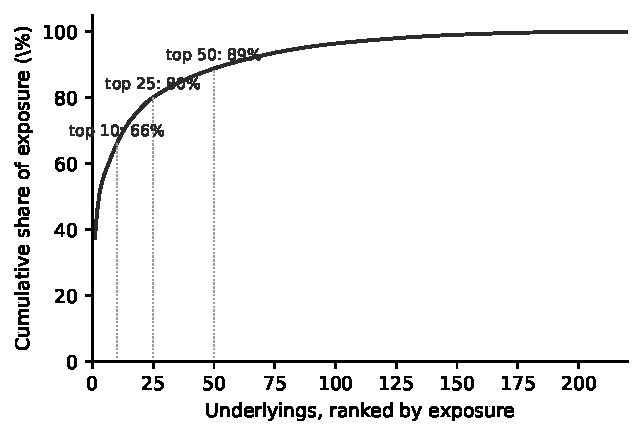
\includegraphics[width=0.49\textwidth]{figures/concentration.pdf}\hfill
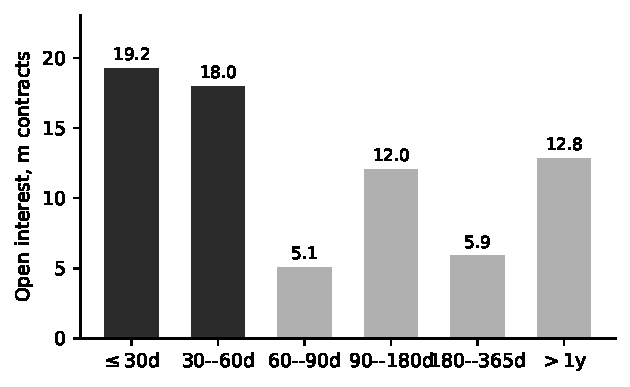
\includegraphics[width=0.49\textwidth]{figures/maturity.pdf}
\caption{Left: cumulative share of open interest by underlying on the final date, ranked.
Right: open interest by remaining maturity. The market is concentrated and more than
half of it expires within sixty days.}
\label{fig:structure}
\end{figure}

\section{Two measurement results}

\subsection{Identifying FLEX without the authoritative report}

Listed strikes fall on a standard grid of whole dollars, halves and quarters, which
suggests treating an off-grid strike as FLEX. Table~\ref{tab:confusion} scores that
rule against the report over 486,895 cleared series.

\begin{table}[t]
\centering
\caption{The off-grid heuristic against the authoritative FLEX report.}
\label{tab:confusion}
\begin{tabular}{lrr}
\toprule
& True FLEX & Not FLEX \\
\midrule
Off-grid strike & 4,914 & 2,389 \\
On-grid strike & 9,321 & 470,271 \\
\midrule
\multicolumn{3}{l}{Precision $0.673$ \quad Recall $0.345$ \quad $F_1$ $0.456$} \\
\bottomrule
\end{tabular}
\end{table}

The rule misses 9,321 FLEX series, 65.5\% of the FLEX in that universe, because FLEX is
routinely struck on the grid --- a series such as \texttt{1AAON} at \$99.00 is FLEX at a
round strike and no strike-based test can find it. A third of what the rule flags is
not FLEX at all.

The consequence for anyone tempted by the same reasoning is that a strike-based
identification of FLEX is not merely noisy but severely biased, and the bias is
invisible without the authoritative source.

\subsection{Cleared series are not economic positions}

Open interest is reported per series. Positions span series. Three cases, each found
while building an earlier census, show what conflating them costs.

\paragraph{A butterfly.} One underlying carries call lines of 100k, 200k and 100k
contracts at equally spaced strikes across three consecutive expiries. Read as nine
independent positions this is \$63.8bn of notional. A butterfly cannot be worth more
than its strike spacing times its wing size: \$1.30bn in total, an overstatement of 49
times.

\paragraph{A collar.} SPY at one expiry carries four legs near 37,500 contracts each ---
a synthetic long, a cap, a floor and a buffer floor. The position is roughly \$2.87bn.
Counted leg by leg at strike-based notional it is \$8.02bn.

\paragraph{A strike-based notional.} The same collar's synthetic long call, struck at
\$1.87 against a spot near \$765, carries \$2.9bn of exposure and is recorded by strike
times contracts as \$7m. Deep in-the-money calls used to replicate an underlying are
three orders of magnitude invisible to that measure, while far out-of-the-money legs
are inflated by it.

The errors have opposite signs and do not cancel. The report's mark prices avoid the
valuation half of the problem directly, since they price each series as cleared.

\section{Does hidden inventory predict the visible market?}

\subsection{Design}

A dealer intermediating a FLEX trade hedges it in the listed market and retains the
residual convexity while the position lives. Inventory observed at $T$, available at
$T+1$, should then inform subsequent behaviour.

Timing is enforced rather than assumed: every predictor is measured at $T$ or earlier
and every outcome strictly after. We estimate
\begin{equation}
y_{i,t+1}
= \alpha_i + \delta_t
+ \beta\,\text{flex}_{i,t}
+ \gamma' \text{controls}_{i,t}
+ \varepsilon_{i,t},
\label{eq:pred}
\end{equation}
with underlying and date fixed effects, errors two-way clustered on both
\citep{cameron2011}, and controls for trailing realised volatility at five and
twenty-two days, the same-day absolute return, and log dollar volume. Inventory enters
as an innovation relative to the underlying's own trailing mean, since its level is
dominated by persistent cross-sectional differences the fixed effects absorb.

The estimation sample is 58,014 underlying-days across 281 underlyings and 231 activity
dates.

\subsection{Result}

\begin{table}[t]
\centering
\caption{Hidden inventory and subsequent realised volatility. MDE80 is the effect
detectable at 80\% power.}
\label{tab:pred}
\begin{tabular}{llrrr}
\toprule
Predictor & Outcome & $\beta$ & $t$ & MDE80 \\
\midrule
Inventory innovation & next-day $|r|$ & $-0.00030$ & $-1.37$ & 0.00062 \\
Inventory change & next-day $|r|$ & $-0.00016$ & $-0.40$ & 0.00115 \\
Near-dated share change & next-day $|r|$ & $+0.00081$ & $+0.58$ & 0.00390 \\
Put share & next-day $|r|$ & $-0.00189$ & $-1.73$ & 0.00307 \\
Inventory innovation & next-day $r^2$ & $-0.00003$ & $-0.81$ & 0.00011 \\
\midrule
\textbf{Placebo: future inventory} & next-day $|r|$ & $\mathbf{-0.00032}$ & $\mathbf{-1.37}$ & 0.00065 \\
\bottomrule
\end{tabular}
\end{table}

Nothing predicts. Longer horizons are weaker still: mean absolute return over the next
three, five and ten days gives $t=-0.88$, $-0.59$ and $-0.12$. Restricting to the top
decile of inventory changes, so that only large creations and extinguishments enter,
gives $t=-0.71$ at one day.

\begin{figure}[t]
\centering
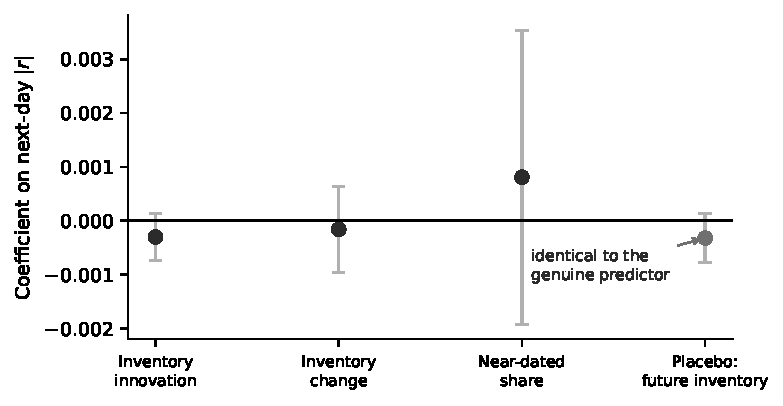
\includegraphics[width=0.68\textwidth]{figures/placebo.pdf}
\caption{Coefficients on next-day absolute return with 95\% intervals. The placebo uses
inventory dated after the outcome and cannot carry information; it is indistinguishable
from the genuine predictor.}
\label{fig:placebo}
\end{figure}

The placebo settles the interpretation (Figure~\ref{fig:placebo}). Using inventory dated \emph{after} the outcome
it is asked to predict --- which cannot carry information --- returns $-0.00032$ at
$t=-1.37$, against the genuine predictor's $-0.00030$ at $t=-1.37$. The association runs
equally well backwards in time, which is the signature of a common factor moving both
series rather than information flowing between them.

\subsection{Power, and what the null does not say}

The minimum detectable effect is roughly $0.0006$ in absolute return against a typical
daily absolute return near $0.02$ in this cross-section, so relative effects of three to
five percent would have been found. The result should be read as a bound at that
resolution rather than as an absence.

Three things are not ruled out, and each would require data that cannot be obtained
retrospectively without cost.

\textbf{Strike-local effects.} Inventory is aggregated to the underlying. If a dealer's
hedging response concentrates at the strikes transacted, aggregation averages it away.
Testing this needs historical strike-level listed implied volatility.

\textbf{Intraday response.} Daily bars cannot see a hedging response completed within a
session.

\textbf{Option-market outcomes.} We predict the underlying. The more natural target is
the listed surface, where a dealer actually lays off risk.

\section{Limitations}

\begin{enumerate}
\item \textbf{Gross, unsigned inventory.} Open interest does not identify who is long,
and is aggregated across holders. No measure here is a dealer position.
\item \textbf{Thirteen months.} The panel is bounded by OCC's retention.
\item \textbf{One outcome family.} Realised volatility in the underlying, not the option
surface.
\item \textbf{No structure decomposition in the panel.} The measurement section shows
that positions span series; the predictive tests use per-underlying aggregates and
inherit none of that decomposition.
\end{enumerate}

\section{Conclusion}

The FLEX market is publicly reported, larger than its absence from chain data suggests,
and growing quickly: open interest roughly doubled over thirteen months to 73 million
contracts, with \$596bn of mark value, concentrated in a few underlyings and more than
half of it expiring within sixty days.

Whether it tells us anything about the visible market is a separate question, and at
the resolution available the answer is no. Per-underlying hidden inventory does not
predict subsequent realised volatility, and a placebo that cannot carry information
performs identically. We regard that as the more useful result to report, because the
marginal coefficient it displaces is exactly the kind that survives into the literature
when no placebo is run.

Two measurement findings travel further than the setting. A natural strike-based rule
for identifying FLEX recovers a third of it. And cleared series are not economic
positions --- a distinction worth three orders of magnitude in one of the cases here,
with errors that do not cancel.

\section*{Declaration}

The research question, empirical design, and all conclusions are the author's own.
Generative AI assistance was used in a supporting capacity for literature search, code
scaffolding, and copy-editing; all such output was verified by the author, who takes
full responsibility for the content of this paper.

\section*{Data and code availability}

Every input is free and public. Collection infrastructure, the panel builder, the
tests, and results as they were produced --- including figures later superseded by the
authoritative report --- are available at the project repository.

\begin{thebibliography}{99}

\bibitem[Bollen and Whaley(2004)]{bollen2004}
Bollen, N.~P.~B. and R.~E. Whaley (2004).
Does net buying pressure affect the shape of implied volatility functions?
\emph{Journal of Finance} 59(2), 711--753.

\bibitem[Cameron et al.(2011)]{cameron2011}
Cameron, A.~C., J.~B. Gelbach, and D.~L. Miller (2011).
Robust inference with multiway clustering.
\emph{Journal of Business and Economic Statistics} 29(2), 238--249.

\bibitem[G\^{a}rleanu et al.(2009)]{garleanu2009}
G\^{a}rleanu, N., L.~H. Pedersen, and A.~M. Poteshman (2009).
Demand-based option pricing.
\emph{Review of Financial Studies} 22(10), 4259--4299.

\bibitem[Ni et al.(2005)]{ni2005}
Ni, S.~X., N.~D. Pearson, and A.~M. Poteshman (2005).
Stock price clustering on option expiration dates.
\emph{Journal of Financial Economics} 78(1), 49--87.

\bibitem[Park and Kurucak(2025)]{park2025}
Park, T. and U.~Kurucak (2025).
Growth of income funds and death of volatility.
Working paper, University of Texas at Dallas.

\end{thebibliography}

\end{document}
